\chapter{Non-deterministic PI}

Pair-Interaction automaton that Nasilowski proposed is deterministic, and it might be considered to be its advantage.

The pair-interaction leads 

The collisions usually lead to the maximal change of the state, which minimizes the viscosity, as we previously discussed.
Moreover, it offers theoretical ground for using Gibbs distribution \ref{gibbs} in derivation of hydrodynamic equations.

\bigskip

But let us explore following examples.
First, consider node with one standing particle.
\begin{figure}[h]
 \centering 
 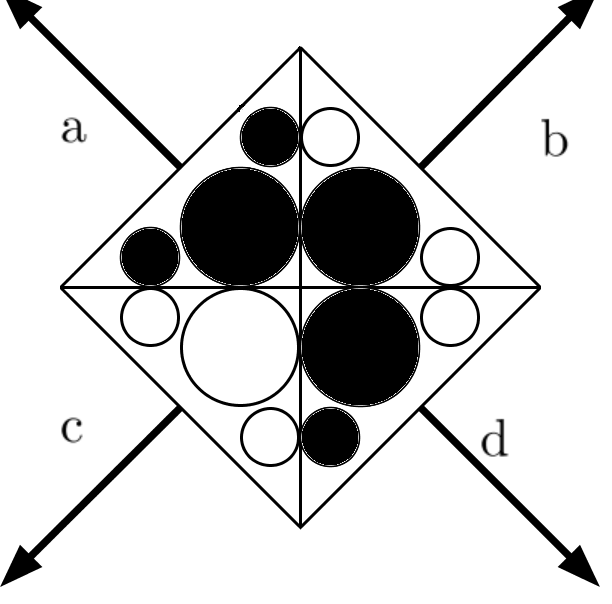
\includegraphics[width=0.22\textwidth]{../nonPInode/node_1}
 \label{transitions}
 \caption{Node before collision}
\end{figure}

By deterministic pair-interactions in X,Y and Z direction, it is always resolved into the state
\begin{figure}[h]
 \centering 
 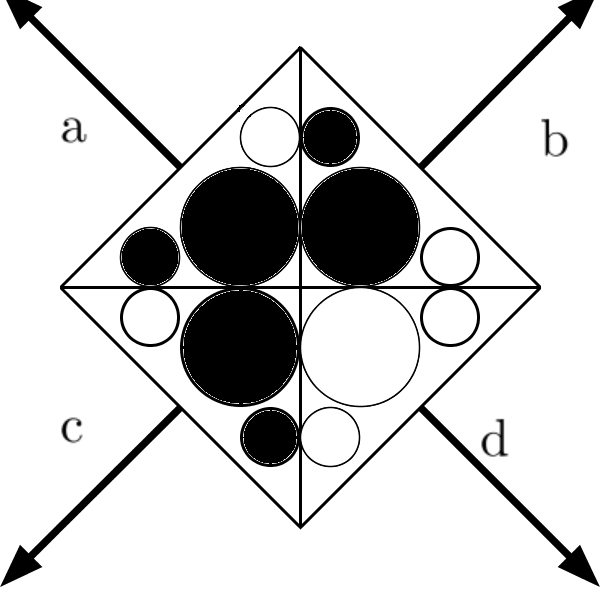
\includegraphics[width=0.22\textwidth]{../nonPInode/node_2}
 \label{transitions}
 \caption{Node after deterministic collision}
\end{figure}

But it is no better then

\begin{figure}[h]
 \centering 
 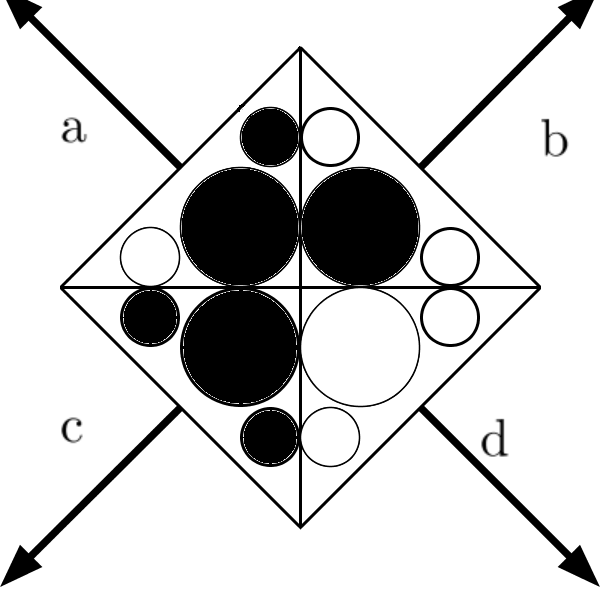
\includegraphics[width=0.22\textwidth]{../nonPInode/node_3}
 \label{transitions}
 \caption{Another acceptable state after collision}
\end{figure}

or any other state with one standing particle.

\bigskip
\newpage
Even better example is the node with two particles with momenta in X direction.
\begin{figure}[htbp]
 \centering 
 \includegraphics[width=0.28\textwidth]{../nonPInode/mom1}
 \label{transitions}
 \caption{Node before collision, and after deterministic collision}
\end{figure}

Deterministic collision do not change its state (pair interaction in Y direction, followed by pair interaction in Z direction leads to the same state for this particular example).

However, collision that would be non-deterministic can lead to the following state
\begin{figure}[htbp]
 \centering 
 \includegraphics[width=0.28\textwidth]{../nonPInode/mom2}
 \label{transitions}
 \caption{Node after non-deterministic collision}
\end{figure}

where both particles gained additional momenta, one in Z, and other in -Z direction.
We could continue with the examples showing deterministic PI do not realize all available states, although some of them are more desirable. 


%Also, we believe that relaxation towards equilibrium might work faster and lead to better results when statistical properties of the flow are inspected.

\bigskip

On the other hand, non-deterministic model, has an obvious drawback. Generation of the random numbers significantly slows the collisions.

To speed up the generation of random number, we hard-coded \textit{Marsaglia's xorshift} generator \cite{mars}, which significantly improved performance comparing to $rand()$ function of C. It may not be appropriate for serious Monte-Carlo simulations, but it is more then enough for our purpose.

\begin{lstlisting}
static unsigned long x=123456789, y=362436069, z=521288629;

unsigned long xorshf96(void) {        
	unsigned long t;
	x ^= x << 16;
	x ^= x >> 5;
	x ^= x << 1;
    t = x;
	x = y;
	y = z;
	z = t ^ x ^ y;

	return z;
}
\end{lstlisting}

\section{Non-deterministic collision}
At the beginning of collision we generate random number by \lstinline|long rand = xorshf96()|.
Before each pair-interaction, we bit-wise shift this number \lstinline|rand >>= 1| , and read the first bit. If it is 1, pair-interaction is performed, otherwise it is skipped.
\begin{lstlisting}
void collision(Node &node)
{
	int d, u;
	unsigned char l, r, ml, mr, lu, ld, ru, rd, li, ri;
	
	// we generate random long
	long rand = xorshf96();
	
	for (int i = 0; i < 3; ++i)
	{
		d = (i + 1) % 3;
		u = (i + 2) % 3;
		for (int j = 0; j < 4; ++j)
		{
			l = Pair[i][j][0];
			r = Pair[i][j][1];

			ml = node.m&l;
			mr = node.m&r;
			ld = node.p[d] & l;
			lu = node.p[u] & l;
			li = node.p[i] & l;
			rd = node.p[d] & r;
			ru = node.p[u] & r;
			ri = node.p[i] & r;

			/* PAIR INTERACTIONS */
			if (!ml && !mr)
				continue;
			if (ml && mr)
			{
				// alternate momenta in direction of the pair-interaction
				if (!ld && !rd)
				{
					//we shift the random number, to the right, and look at the first bit
					rand >>= 1;
					if(rand & 1)
					{
						//if the first bit is 1, the pair-interaction is performed
						node.p[d] |= l;
						node.p[d] |= r;
					}
				}
				else if (ld && rd)
				{
					rand >>= 1;
					if(rand & 1)
					{
						node.p[d] ^= l;
						node.p[d] ^= r;
					}
				}
				// alternate momenta in all other directions
				if (lu && !ru)
				{
					rand >>= 1;
					if(rand & 1)
					{
						node.p[u] ^= l;
						node.p[u] |= r;
					}
				}
				else if (!lu && ru)
				{
					rand >>= 1;
					if(rand & 1)
					{
						node.p[u] |= l;
						node.p[u] ^= r;
					}
				}
				if (li && !ri)
				{
					rand >>= 1;
					if(rand & 1)
						continue;
					node.p[i] ^= l;
					node.p[i] |= r;
				}
				else if (!li && ri)
				{
					rand >>= 1;
					if(rand & 1)
						continue;
					node.p[i] |= l;
					node.p[i] ^= r;
				}
			}
			else if (!ml && !rd)
			{
				rand >>= 1;
				if(rand & 1)
					continue;
				node.m |= l;
				node.m ^= r;
				if (ru)
				{
					node.p[u] |= l;
					node.p[u] ^= r;
				}
				if (ri)
				{
					node.p[i] |= l;
					node.p[i] ^= r;
				}					
			}
			else if (!mr && !ld)
			{
				rand >>= 1;
				if(rand & 1)
					continue;
				node.m |= r;
				node.m ^= l;
				if (lu)
				{
					node.p[u] |= r;
					node.p[u] ^= l;
				}
				if (li)
				{
					node.p[i] |= r;
					node.p[i] ^= l;
				}
			}
		}
	}
}
\end{lstlisting}

\section{Exploding cube}
To demonstrate the difference of deterministic and non-deterministic automaton in the crystal form, we simulated the "explosion of the cube". 

The simulations were performed on the lattice $240 \cross 240 \cross 240$ with periodic boundary conditions.
Into the cube with side 3 times smaller then the size of lattice (thus containing $1/27$ of all nodes), we put particles with zero momentum in all available cells.

The evolution of the system for both versions of PI is to be seen on the following pictures.
\begin{figure}[H]
 \centering 
 \includegraphics[width=0.9\textwidth]{../cubedeter/velocity_0}
 \caption{Deterministic PI - time 0}
\end{figure}

\begin{figure}[H]
 \centering 
 \includegraphics[width=0.9\textwidth]{../cubenon/velocity_0}
 \caption{Non-deterministic PI - time 0}
\end{figure}

\begin{figure}[H]
 \centering 
 \includegraphics[width=0.9\textwidth]{../cubedeter/velocity_20}
 \caption{Deterministic PI - time 20}
\end{figure}

\begin{figure}[H]
 \centering 
 \includegraphics[width=0.9\textwidth]{../cubenon/velocity_20}
 \caption{Non-deterministic PI - time 20}
\end{figure}

\begin{figure}[H]
 \centering 
 \includegraphics[width=0.9\textwidth]{../cubedeter/velocity_50}
 \caption{Deterministic PI - time 50}
\end{figure}

\begin{figure}[H]
 \centering 
 \includegraphics[width=0.9\textwidth]{../cubenon/velocity_50}
 \caption{Non-deterministic PI - time 50}
\end{figure}

\begin{figure}[H]
 \centering 
 \includegraphics[width=0.9\textwidth]{../cubedeter/velocity_80}
 \caption{Deterministic PI - time 80}
\end{figure}

\begin{figure}[H]
 \centering 
 \includegraphics[width=0.9\textwidth]{../cubenon/velocity_80}
 \caption{Non-deterministic PI - time 80}
\end{figure}

\begin{figure}[H]
 \centering 
 \includegraphics[width=0.9\textwidth]{../cubedeter/velocity_110}
 \caption{Deterministic PI - time 110}
\end{figure}

\begin{figure}[H]
 \centering 
 \includegraphics[width=0.9\textwidth]{../cubenon/velocity_110}
 \caption{Non-deterministic PI - time 110}
\end{figure}

\begin{figure}[H]
 \centering 
 \includegraphics[width=0.9\textwidth]{../cubedeter/velocity_140}
 \caption{Deterministic PI - time 140}
\end{figure}

\begin{figure}[H]
 \centering 
 \includegraphics[width=0.9\textwidth]{../cubenon/velocity_140}
 \caption{Non-deterministic PI - time 140}
\end{figure}

\begin{figure}[H]
 \centering 
 \includegraphics[width=0.9\textwidth]{../cubedeter/velocity_160}
 \caption{Deterministic PI - time 160}
\end{figure}

\begin{figure}[H]
 \centering 
 \includegraphics[width=0.9\textwidth]{../cubenon/velocity_160}
 \caption{Non-deterministic PI - time 160}
\end{figure}

\begin{figure}[H]
 \centering 
 \includegraphics[width=0.9\textwidth]{../cubedeter/velocity_180}
 \caption{Deterministic PI - time 180}
\end{figure}

\begin{figure}[H]
 \centering 
 \includegraphics[width=0.9\textwidth]{../cubenon/velocity_180}
 \caption{Non-deterministic PI - time 180}
\end{figure}

\begin{figure}[H]
 \centering 
 \includegraphics[width=0.9\textwidth]{../cubedeter/velocity_220}
 \caption{Deterministic PI - time 220}
\end{figure}

\begin{figure}[H]
 \centering 
 \includegraphics[width=0.9\textwidth]{../cubenon/velocity_220}
 \caption{Non-deterministic PI - time 220}
\end{figure}

\begin{figure}[H]
 \centering 
 \includegraphics[width=0.9\textwidth]{../cubedeter/velocity_260}
 \caption{Deterministic PI - time 260}
\end{figure}

\begin{figure}[H]
 \centering 
 \includegraphics[width=0.9\textwidth]{../cubenon/velocity_260}
 \caption{Non-deterministic PI - time 260}
\end{figure}

\begin{figure}[H]
 \centering 
 \includegraphics[width=0.9\textwidth]{../cubedeter/velocity_300}
 \caption{Deterministic PI - time 300}
\end{figure}

\begin{figure}[H]
 \centering 
 \includegraphics[width=0.9\textwidth]{../cubenon/velocity_300}
 \caption{Non-deterministic PI - time 300}
\end{figure}

\begin{figure}[H]
 \centering 
 \includegraphics[width=0.9\textwidth]{../cubedeter/velocity_322}
 \caption{Deterministic PI - time 0}
\end{figure}

\begin{figure}[H]
 \centering 
 \includegraphics[width=0.9\textwidth]{../cubenon/velocity_322}
 \caption{Non-deterministic PI - time 0}
\end{figure}

%The is only short excerpt of the evolution of deterministic PI. 
The patterns that you see for deterministic PI were repeating in the infinite loop. We performed simulation up to 9000 steps and the pattern did not change.

On the other hand, the pattern in the non-deterministic PI broke after the first explosion already and exhibits the realistic "spilling" of the particles, in contrast to the perfect periodic evolution of deterministic automaton.
